% This file was created by tikzplotlib v0.9.8.
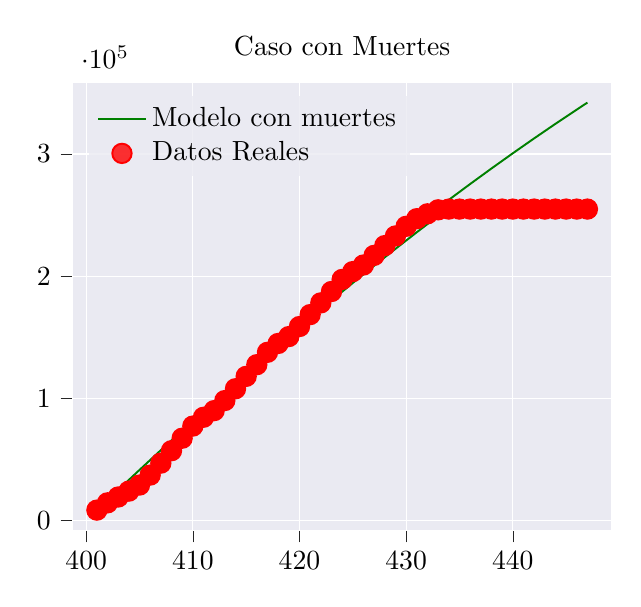
\begin{tikzpicture}

\definecolor{color0}{rgb}{0.917647058823529,0.917647058823529,0.949019607843137}

\begin{axis}[
axis background/.style={fill=color0},
axis line style={white},
legend cell align={left},
legend style={
  fill opacity=0.8,
  draw opacity=1,
  text opacity=1,
  at={(0.03,0.97)},
  anchor=north west,
  draw=none,
  fill=color0
},
tick align=outside,
tick pos=left,
title={Caso con Muertes},
x grid style={white},
xmajorgrids,
xmin=398.7, xmax=449.3,
xtick style={color=white!15!black},
y grid style={white},
ymajorgrids,
ymin=-8365.24688698199, ymax=358820.184626622,
ytick style={color=white!15!black}
]
\addplot [line width=0.7pt, green!50!black]
table {%
401 8325
403 24862.265625
405 41240.765625
407 57450.734375
409 73482.8671875
411 89328.3203125
413 104978.734375
415 120426.2578125
417 135663.515625
419 150683.65625
421 165480.375
423 180047.828125
425 194380.734375
427 208474.296875
429 222324.25
431 235926.84375
433 249278.78125
434 255859.875
434 262440.96875
436 275411.875
438 288126.0625
440 300581.9375
442 312778.28125
444 324714.375
446 336389.90625
447 342129.9375
};
\addlegendentry{Modelo con muertes}
\addplot [line width=0.7pt, red, mark=*, mark size=3.5, mark options={solid}, only marks]
table {%
401 8325
402 14302
403 19083
404 23893
405 28852
406 37027
407 46810
408 57008
409 67214
410 77152
411 84377
412 89813
413 98062
414 107740
415 117881
416 127446
417 137577
418 144822
419 150471
420 158701
421 168455
422 178076
423 187374
424 197274
425 203682
426 209100
427 216969
428 225001
429 232869
430 240780
431 247016
432 251005
433 254278
434 254890
435 254890
436 254890
437 254890
438 254890
439 254890
440 254890
441 254890
442 254890
443 254890
444 254890
445 254890
446 254890
447 254890
};
\addlegendentry{Datos Reales}
\end{axis}

\end{tikzpicture}
